\documentclass[a4paper]{article}
\usepackage{geometry}
\usepackage{graphicx}
\usepackage{hyperref}
\usepackage{amsmath}

% \input{/Users/wsaleem/Courses/CS412/wc/pythonhighlight.sty}
% \usepackage{pythonhighlight}
% \usepackage{titling}

% \usepackage{draftwatermark}
% \SetWatermarkText{Sample Solution}
% \SetWatermarkScale{3}
% \printanswers

\title{Weekly Challenge 06 (Group): Divide and Conquer Multiplication}
\author{CS/CE 412/471 Algorithms: Design and Analysis}
\date{Spring 2025}

% \qformat{{\large\bf \thequestion. \thequestiontitle}\hfill}
% \boxedpoints

\begin{document}
\maketitle
\thispagestyle{empty}
\begin{center}
Total points: 25
\end{center}
\section*{Objective}
In this WC, you will work in groups and:
\begin{itemize}
\item understand and modify a divide-and-conquer algorithm to multiply 2 n-digit numbers efficiently 
\item demonstrate step-by-step working with examples and hand-drawn illustrations.
\item derive recurrence relations from the given algorithm 
\item solve recurrence relations using methods like substitution, recursion trees, and/or the Master Theorem,
\end{itemize}

\section*{Motivation}

 Traditional methods of multiplication like the one we learned in grade 3, become inefficient for large numbers, making divide-and-conquer approaches more effective. This challenge enhances understanding of such techniques by understanding, modifying, and analyzing the algorithm Multiply-Binary, helping students revisit recursion, recurrence relations, and time complexity calculations.

\newpage
\section{Multiply-Binary} \label{sec:binary}
Consider the following divide-and-conquer algorithm which multiplies 2 n-bit \textbf{binary} numbers using divide-and-conquer:
\\
\\
\noindent\textbf{Algorithm:} \textsc{Multiply-Binary}$(x, y)$  
\\
\textbf{Input:} 2 positive binary integers $x$ and $y$
\\
\textbf{Output:} Their product $x * y$

\begin{enumerate}
    \item $n = \max(\text{size of } x, \text{size of } y)$
    \item \textbf{if} $n = 1$ \textbf{then return} $x * y$
    \item $m = \lfloor n / 2 \rfloor$
    \item $x_L = \lfloor x / 2^m \rfloor, \quad x_R = x \mod 2^m$
    \item $y_L = \lfloor y / 2^m \rfloor, \quad y_R = y \mod 2^m$
    \item $P_1 = \textsc{Multiply-Binary}(x_L, y_L)$
    \item $P_2 = \textsc{Multiply-Binary}(x_R, y_R)$
    \item $P_3 = \textsc{Multiply-Binary}(x_L + x_R, y_L + y_R)$
    \item \textbf{return} $P_1 \cdot 2^n + (P_3 - P_1 - P_2) \cdot 2^m + P_2$
\end{enumerate}

\begin{figure}[h!]
    \centering
    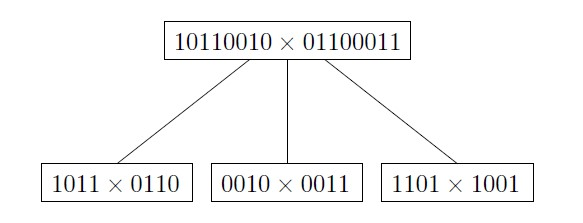
\includegraphics[width=0.5\textwidth]{binary.jpg}
    \caption{Instance of a Recursion Tree showing how a size-n multiplication problem is divided into size-n/2 sub-problems. How many sub-problems do you see?}
    \label{fig:example}
\end{figure}


\subsection{Working Example (5 points)}
Demonstrate a working example of Procedure Multiply-Binary using any 2 4-bit numbers. Include figure of your hand-written working.

\newpage
\section{Multiply-Decimal}
We need to modify the algorithm Multiply-Binary considering if the inputs and outputs are now decimal numbers.

\subsection{Procedure Multiply-Decimal  (5 points)}
Write the pseudo-code for Procedure Multiply-Decimal in CLRS notation. No credit if you use any programming language constructs or methods e.g. list.append(), etc. 

\subsection{Working Example (5 points)}
Demonstrate a working example of Procedure Multiply-Decimal using any 2 4-digit numbers. Include figure of your hand-written working.

\subsection{Recurrence (5 points)}
Devise a recurrence for the designed algorithm Procedure Multiply-Decimal.

\subsection{Time Complexity (5 points)}
Solve the recurrence using the master method to find the Time Complexity of the algorithm.

\section*{Submission}
\begin{enumerate}
\item Submit one pdf file including your solutions. 
\item Clearly write your group number, member names and ids. \item Where a working examples are required, you should include a hand-written working snapshot that demonstrates the step-wise working of the procedure.
\end{enumerate}

\end{document}

%%% Local Variables:
%%% mode: latex
%%% TeX-master: t
%%% End:
